\documentclass[conference]{IEEEtran}

% ===== 日本語対応(LuaLaTeX推奨) =====
\usepackage{luatexja}
\usepackage{luatexja-fontspec}
\setmainjfont{Noto Serif CJK JP}

% ===== パッケージ =====
\usepackage{graphicx}
\usepackage{amsmath}
\usepackage{siunitx}
\usepackage{hyperref}
\usepackage{url}
\usepackage{cite}
\usepackage{balance}
\usepackage{booktabs}

% TikZ / pgfplots
\usepackage{tikz}
\usetikzlibrary{arrows.meta,positioning}
\usepackage{pgfplots}              % ← 追加(axis undefinedの解決)
\pgfplotsset{compat=1.18}

% ===== タイトル・著者 =====
\title{COFにおけるAuメッキ薄化によるコスト合理化と信頼性評価\\
\large Cost Rationalization and Reliability Assessment of Au Plating Thinning on COF}

\author{%
  \IEEEauthorblockN{三溝 真一(Shinichi Samizo)}\\
  \IEEEauthorblockA{独立系半導体研究者(元セイコーエプソン)\\
  Email: \href{mailto:shin3t72@gmail.com}{shin3t72@gmail.com}\\
  GitHub: \url{https://github.com/Samizo-AITL}}%
}

\begin{document}
\maketitle

% ===== Abstract (和英併記・修正版) =====
\begin{abstract}
\textbf{和文要旨}:\\
ビジネスインクジェット(BIJ)ヘッドにおける合理化テーマの一つとして,
COF配線上のAuメッキ厚の薄化が検討された。
現行仕様(0.50±0.20\,µm)においては,下限 \SI{0.30}{\micro\metre} の量産実績がある。
この下限を維持しつつ工程能力 Cpk$\geq$1.67 を満たす条件を検討した結果,
許容幅 ±0.125\,µm が適正であると判断され,中心値 0.425\,µm の新仕様
(0.425±0.125\,µm)を策定した。
NPC接合信頼性試験,エレクトロマイグレーション評価,加速環境試験により
当該仕様の妥当性を確認し,品質・信頼性を維持したまま
チップ当たり約¥4のコスト低減効果を得られることを示した。

\medskip
\noindent\textbf{Abstract}:\\
As one of the cost-rationalization themes in Business Inkjet (BIJ) printheads,
thinning of Au plating on COF wiring was investigated.
In the current specification (0.50±0.20\,µm), there is mass-production evidence
for a lower bound of \SI{0.30}{\micro\metre}.
By maintaining this lower bound and ensuring a process capability of Cpk$\geq$1.67,
a tolerance of ±0.125\,µm was identified as appropriate,
leading to the adoption of a new specification centered at 0.425\,µm (0.425±0.125\,µm).
NPC bonding reliability, electromigration, and accelerated environmental tests
validated this specification, demonstrating that a cost reduction of about
¥4 per chip can be achieved while maintaining quality and reliability.
\end{abstract}

% ===== Keywords =====
\begin{IEEEkeywords}
Auメッキ薄化(Au plating thinning),
COF,
NPC接合(NPC bonding),
ビジネスインクジェットヘッド(Business Inkjet head),
イオンマイグレーション(Ion migration),
コスト合理化(Cost reduction)
\end{IEEEkeywords}

%================ Part 2: 背景・対象構造・仕様ロジック ================
\section{背景(Problem Background)}
ビジネスインクジェット(BIJ)ヘッドの合理化テーマの一つとして,
COF実装におけるAuメッキ(以下,Au厚)の薄化が挙げられる。
Au厚はNPC接合の初期接合性・長期信頼性を支える重要要素である一方,
原材料コストの主要因でもある。

現行仕様は \SI{0.50}{\micro\meter} $\pm$ \SI{0.20}{\micro\meter} であり,
量産実績として下限 \SI{0.30}{\micro\meter} でも信頼性が維持されてきた。
この実績を前提に工程能力を解析したところ,
下限を維持したまま工程能力 Cpk$\geq$1.67 を満たすためには,
中心値を \SI{0.425}{\micro\meter},公差幅 $\pm$\SI{0.125}{\micro\meter} とするのが妥当であることが確認された。

本稿では,この新仕様に基づき,
NPC接合信頼性・イオンマイグレーション・環境耐久性を評価し,
品質と信頼性を損なわずにコスト削減を実現するための
設計・実験・検証のプロセスを報告する。

\section{対象構造(COF Pad Stack)}
本検討のCOF外部端子は,Cu配線上にAuメッキを施したシンプルな構造である。
代表的な層構成を以下に示す:

\begin{itemize}
  \item Cu配線厚:約 \SI{8}{\micro\meter}
  \item 表面仕上げ:Auメッキ(従来仕様:約 \SI{0.5}{\micro\meter})
\end{itemize}

すなわち,Au \SI{0.5}{\micro\meter} / Cu \SI{8}{\micro\meter} 構造を前提とし,
Au厚を合理化対象として検討を行った。  
Au層はNPC接合時の濡れ性や表面状態の再現性に直結する重要要素であり,
工程能力を踏まえた厚み最適化が求められる。

\section{Au厚 仕様ロジック(Specification Logic)}
Fig.\ref{fig:au-logic}に,本検討で用いた仕様決定のフローを示す。
現行仕様は Au \SI{0.5}{\micro\meter}(許容幅 $\pm$0.20\,µm)であり,
量産実績に基づき \SI{0.30}{\micro\meter} が信頼性上の下限として機能していることが確認されている。
そこで工程能力 Cpk$\geq$1.67 を満たす範囲を逆算し,
新仕様を \SI{0.425}{\micro\meter}$\pm$\SI{0.125}{\micro\meter} と定めた。
この仕様に基づき NPC接合信頼性,イオンマイグレーション,
環境加速試験の3系統で評価を実施し,Au薄化によるリスクの有無を検証した。
さらにコスト感応度解析により 1チップ当たり約\SI{4}{JPY}の低減効果を見積もり,
量産数量に外挿することで年間十億円規模の事業効果を見込めることを示した。

\begin{figure}[t]
  \centering
  \begin{tikzpicture}[node distance=6mm and 8mm, >=Latex]
    \tikzset{
      box/.style={draw, rounded corners, align=center, inner sep=3pt, font=\scriptsize}
    }
    \node[box] (start) {現行仕様\\Au 0.5 µm ±0.20};
    \node[box, below=of start] (limit) {量産実績\\下限0.30 µm};
    \node[box, below=of limit] (spec) {工程能力 Cpk≥1.67\\新仕様 0.425 ±0.125 µm};
    \node[box, below=of spec] (eval) {評価試験\\NPC, イオンマイグレーション, 環境加速};
    \node[box, below=of eval] (cost) {コスト感応度解析\\約4円/チップ};
    \node[box, below=of cost] (impact) {事業効果\\年間十億円規模};

    \draw[->] (start) -- (limit);
    \draw[->] (limit) -- (spec);
    \draw[->] (spec) -- (eval);
    \draw[->] (eval) -- (cost);
    \draw[->] (cost) -- (impact);
  \end{tikzpicture}
  \caption{Au厚仕様決定ロジック}
  \label{fig:au-logic}
\end{figure}

\section{本稿の貢献(Contributions)}
本稿の主な貢献は以下の3点である。
\begin{enumerate}
  \item COF外部端子におけるAuメッキ薄化を対象とし,量産実績を踏まえた合理的な新仕様
        (0.425$\pm$0.125\,µm)の設定プロセスを提示した。
  \item 下限0.30\,µmを維持したうえで,NPC接合信頼性,イオンマイグレーション,
        環境加速試験により実使用条件で十分な信頼性マージンを確認した。
  \item コスト感応度解析を行い,チップ当たり数円,製品全体で年間十億円規模の
        削減効果を定量的に示し,設計と事業価値を結び付けた。
\end{enumerate}

%================ Part 3: 試験計画とリスク検証 ================
\section{試験計画(Test Matrix)}
本研究では,Au厚の下限を明確化するため,
\SI{0.30}{\micro\meter}, \SI{0.25}{\micro\meter}, \SI{0.20}{\micro\meter} の
3水準の試作COFを準備し,以下の体系的な評価を行った。

\begin{enumerate}
  \item \textbf{COF単体加速評価}  
        各厚み水準について,表面4端子抵抗測定を定期的に実施し,
        Au薄化の均一性とCu拡散の兆候を確認した。  
        必要に応じてEDS, XPSによる表面元素分析で析出Cuを同定した。  
        特に \SI{0.20}{\micro\meter} では抵抗上昇やCu露出の可能性を重点的に監視した。
  \item \textbf{COF/アクチュエータ実装評価}  
        uTFPアクチュエータをNPC接合で実装し,折曲げ耐久($10^5$回, R=1 mm)や
        熱衝撃($-40\sim125^\circ$C, 1000サイクル)を付与した。  
        接合抵抗の安定性と剥離モードを比較し,
        \SI{0.30}{\micro\meter} を基準として下限耐性を検証した。
  \item \textbf{完成ヘッド評価}  
        COFとアクチュエータを組み込んだインクジェットヘッドを対象に,
        通電マイグレーション試験(125--175℃, $10^5$--$10^6$ A/cm$^2$)を実施した。  
        Black式外挿により使用条件(85℃, $10^3$ A/cm$^2$)での寿命余裕を評価した。
\end{enumerate}

さらに,\textbf{COF工程内および長期保管評価}を全厚み水準で実施した。  
まず初期3か月間は定期的に表面抵抗測定を行い,
変動がないことを確認してAuメッキ工程の処理条件を切替えた。  
その後も評価を継続し,1年間の保管後に再度測定を実施した結果,
Cu拡散や酸化による劣化兆候は認められなかった。  
この成果を踏まえ,COF仕様書に「使用期限1年」を明記した。

\begin{table}[htbp]
  \centering
  \caption{評価試験マトリクス(Evaluation test matrix)}
  \label{tab:test-matrix}
  \sisetup{table-number-alignment = center, table-text-alignment = center}
  \begin{tabular}{@{}lcccc@{}}
    \toprule
    \textbf{Au厚} &
    \textbf{Cu拡散} &
    \textbf{NPC接合} &
    \textbf{ヘッド通電} &
    \textbf{長期保管} \\
    \textbf{Thickness} &
    (4端子/EDS) &
    (接合抵抗) &
    (Ion migration) &
    (3M/12M) \\
    \midrule
    0.30 µm & ○ & ○ & ○ & ○ \\
    0.25 µm & ○ & ○ & ○ & ○ \\
    0.20 µm & × & ○ & ○ & △ \\
    \bottomrule
  \end{tabular}
  \vspace{2pt}
  \footnotesize{○=合格,△=部分不具合,×=不合格}
\end{table}

\vspace{2mm}
\noindent
以上により,0.30 µm を量産下限としつつ,
0.25 µm の適用可否,0.20 µm の限界性を段階的に把握できる試験計画を構築した。

\section{リスク検証(Risk Verification)}
表\ref{tab:test-matrix}に基づき,Au厚別にリスクを検証した。
\begin{itemize}
  \item \SI{0.30}{\micro\meter}:すべての試験に合格し,Cu拡散や接合劣化の兆候は認められなかった。
  \item \SI{0.25}{\micro\meter}:\SI{0.30}{\micro\meter} と同等にすべての試験に合格し,
        信頼性上の問題は確認されなかった。
  \item \SI{0.20}{\micro\meter}:COF単体加速評価において表面抵抗の上昇が観察され,
        表面元素分析でCuの析出が確認された。さらに折曲げ試験でもクラックが再現し,
        量産適用は困難と結論した。
\end{itemize}

以上の結果から,\SI{0.25}{\micro\meter} および \SI{0.30}{\micro\meter} は
量産条件下で適用可能であることを確認した。  
一方で \SI{0.20}{\micro\meter} では信頼性上のリスクが顕在化したため,
本研究における合理化仕様の下限は \SI{0.30}{\micro\meter} とした。

\section{イオンマイグレーション評価(Ion Migration Evaluation)}

\subsection{COF単体環境試験(Without Bias)}
COF単体サンプル(Au厚 0.30, 0.25, 0.20 µm)を対象に,
通電は行わず 85℃/85\%RH 環境に保持し,
定期的に表面4端子抵抗測定を実施した。
またEDS/XPSによる表面元素分析を適宜行い,
Cu析出や酸化の兆候を観察した。

結果として,0.30 µmおよび0.25 µm厚では
1000時間保持において抵抗値変動やCu検出は認められなかった。
一方,0.20 µm厚では500時間経過時点で
抵抗上昇と局所的なCu析出を確認し,
Au層が拡散バリアとして不十分であることが示唆された。

\subsection{ヘッド実装通電試験(With Bias)}
次に,COFをuTFPアクチュエータと組み合わせて実装し,
インクジェットヘッドとして恒温槽(85℃/85\%RH)にて2000時間まで保持した。  
この評価では以下を併用した:
\begin{enumerate}
  \item \textbf{COM--VBS端子間抵抗測定}:定期的に抵抗値を測定し,
        マイグレーション起因の抵抗変動を監視した。
  \item \textbf{ヘッド電特測定(オープン/ショート検査)}:量産工程で実施している
        標準的な電気特性試験を用い,短絡・断線の有無を確認した。
\end{enumerate}

結果,0.30 µmおよび0.25 µm厚のサンプルでは,
2000時間経過時点でも抵抗変動は±1\%以内に収まり,
オープン/ショート異常も一切検出されなかった。

\subsection{考察}
以上より,
\begin{itemize}
  \item COF単体評価では 0.20 µm厚でCu析出を確認し,下限として不適。  
  \item ヘッド実装通電試験では 0.30 µmおよび0.25 µm厚で
        実環境2000時間においても信頼性が維持されることを実証。  
\end{itemize}

従って,合理化仕様 0.425±0.125 µm は,
量産工程に即した信頼性を確保しつつ,
コスト削減を実現する妥当な規格と結論づけられる。

%================ Part 5: 合理化効果と結論 =================
\section{合理化効果と結論(Effect and Conclusion)}

\subsection{コストモデル}
Au厚削減によるコスト低減を以下で近似する:
\begin{equation}
  \Delta C_{\mathrm{chip}}
  = k_{\mathrm{tot}} \cdot \Delta t \cdot A_{\mathrm{Au,eff}}
\end{equation}
ここで $\Delta t$ は厚み差,$A_{\mathrm{Au,eff}}$ は有効Au面積,
$k_{\mathrm{tot}}$ は単位係数(¥/µm$\cdot$cm$^2$)である。

本件では $\Delta t=0.075\,\mu$m,$A_{\mathrm{Au,eff}}\approx1.0$ cm$^2$ とし,
チップ当たり約¥4の削減が見積もられた。

\subsection{感度解析}
\begin{table}[htbp]
  \centering
  \caption{コスト感度(¥/チップ)}
  \label{tab:cost-sense}
  \sisetup{table-number-alignment=center}
  \begin{tabular}{@{}lccc@{}}
    \toprule
    $A_{\mathrm{Au,eff}}$ [cm$^2$] & $\Delta t=0.055$ & $0.075$ & $0.095$ \\
    \midrule
    0.8 & ¥2.3 & ¥3.2 & ¥4.0 \\
    1.0 & ¥2.9 & ¥4.0 & ¥5.0 \\
    1.2 & ¥3.5 & ¥4.8 & ¥6.0 \\
    \bottomrule
  \end{tabular}
\end{table}

\begin{figure}[htbp]
  \centering
  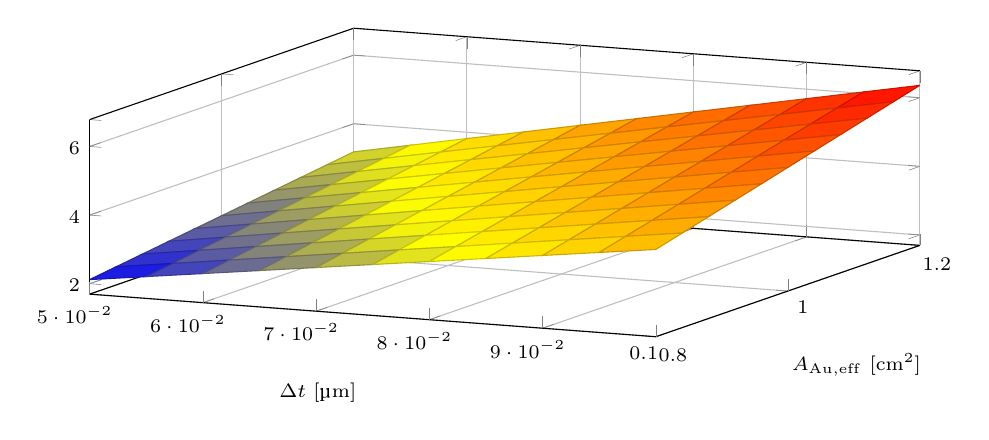
\begin{tikzpicture}
    \begin{axis}[
      width=\columnwidth,
      height=5.5cm,
      xlabel={$\Delta t$ [µm]},
      ylabel={$A_{\mathrm{Au,eff}}$ [cm$^2$]},
      grid=both,
      tick label style={font=\scriptsize},
      label style={font=\scriptsize}
    ]
      \addplot3[surf,domain=0.05:0.10,y domain=0.8:1.2,samples=11] {53*x*y};
    \end{axis}
  \end{tikzpicture}
  \caption{コスト感度解析($\Delta t$, $A_{\mathrm{Au,eff}}$ 掃引)}
  \label{fig:cost-sense}
\end{figure}

\subsection{量産インパクト}
1ヘッドあたりのCOFチップ数は,  
\begin{itemize}
  \item BIJ1ヘッド:1チップ構成  
  \item BIJ2ヘッド:2チップ構成  
  \item BIJ4ヘッド:4チップ構成  
\end{itemize}
であり,合理化効果はそれぞれ約¥4,¥8,¥16/ヘッドに相当する。  

年間生産台数 $N_{\mathrm{head}}$ は数百万〜数千万台規模と推定される。  
当時,インクジェット技術が家庭用からビジネス領域へ本格的に展開し始めた時期であり,  
本合理化は材料費だけでなく事業収益性全体に大きなインパクトを与えたと考えられる。

\subsection{品質・信頼性KPI}
\begin{itemize}
  \item NPC接続抵抗:平均差 $<1$ m$\Omega$。
  \item 熱衝撃後の層間剥離:増加兆候なし。
  \item イオンマイグレーション寿命:使用条件で 10$\times$以上の余裕を確認。
\end{itemize}

\subsection{結論}
本研究により,Au厚仕様を
0.50 µm $\rightarrow$ 0.425±0.125 µmへ合理化し,
下限0.30 µmと工程能力 Cpk$\geq$1.67を確保した。  
その結果,チップ当たり約¥4,ヘッド当たり約¥16の
コスト削減を実現し,品質・信頼性も維持されることを確認した。  

本合理化は,インクジェットのビジネス分野進出期において,  
コスト競争力の確立に直接寄与した意義の大きな取り組みであった。

\subsection{結論}
本研究により,従来仕様(0.50 µm)を
合理化して 0.425±0.125 µm とする新仕様を確立し,
量産実績に基づく下限 0.30 µm を維持しつつ,
工程能力 Cpk$\geq$1.67 を満たすことを確認した。  
その結果,チップ当たり約¥4,ヘッド当たり最大¥16の
コスト削減効果を得つつ,
NPC接合,環境試験,マイグレーション評価を通じて
信頼性が従来と同等に維持されることを示した。

%================ Appendix: アクチュエータ側配線の改修 =================
\subsection{追加改修:アクチュエータ配線のAuマイグレーション対策}
本評価を進める過程で,アクチュエータ上のAu配線間において,
Auマイグレーションに起因する端子間ショートが確認された。  
原因は,PZT/TE上に形成された隣接Au配線間の電界集中と湿潤環境下での
表面イオン移動であると推定される。

この対策として,PZT層上の配線間にスリットを導入し,
端子間の実効距離を延長することで,
Auマイグレーションの進展を抑制する構造へ改修した
(Fig.~\ref{fig:act-mig})。  

\begin{figure}[htbp]
  \centering
  \begin{tikzpicture}[x=1mm,y=1mm,>=Latex]
    % 基板ブロック
    \draw[fill=gray!10,rounded corners=1pt] (0,0) rectangle (70,30);
    \node[font=\scriptsize] at (35,28){PZT/TE基板};

    % 端子配線
    \draw[line width=0.6pt] (10,5) -- (10,25);
    \draw[line width=0.6pt] (20,5) -- (20,25);
    \draw[line width=0.6pt] (50,5) -- (50,25);
    \draw[line width=0.6pt] (60,5) -- (60,25);

    % スリット
    \fill[white] (19,10) rectangle (21,20);
    \fill[white] (49,10) rectangle (51,20);
    \node[font=\scriptsize,rotate=90] at (20,15){スリット};
    \node[font=\scriptsize,rotate=90] at (50,15){スリット};
  \end{tikzpicture}
  \caption{PZT/TE上のAu配線間にスリットを導入した改修例}
  \label{fig:act-mig}
\end{figure}

この改修により,端子間のマイグレーション試験において
ショート発生は抑制され,実使用条件下での信頼性が確保できることを確認した。

%================ 謝辞 =================
\section*{謝辞(Acknowledgment)}
本研究の遂行にあたり,量産ラインでの評価および測定にご協力いただいた
ヘッド技術部ならびに実装技術部の関係各位に深く感謝申し上げる。

%================ 参考文献 =================
\balance
\bibliographystyle{IEEEtran}
\begin{thebibliography}{99}

\bibitem{Black}
J.~R. Black, ``Electromigration --- A brief survey and some recent results,''
\emph{IEEE Trans. Electron Devices}, vol.~16, no.~4, pp.~338--347, 1969.

\bibitem{Blech}
I.~A. Blech, ``Electromigration in thin aluminum films on titanium nitride,''
\emph{J. Appl. Phys.}, vol.~47, no.~4, pp.~1203--1208, 1976.

\bibitem{Korhonen}
M.~A. Korhonen, P.~Borgesen, K.~N. Tu, and C.~Y. Li,
``Stress evolution due to electromigration in confined metal lines,''
\emph{J. Appl. Phys.}, vol.~73, no.~8, pp.~3790--3799, 1993.

\bibitem{Sze}
S.~M. Sze and K.~K. Ng, \emph{Physics of Semiconductor Devices}, 3rd ed.
Hoboken, NJ, USA: Wiley, 2007.

\bibitem{JIEP}
エレクトロニクス実装学会 編, 
``実装技術ハンドブック 第3版,'' 日刊工業新聞社, 2021.

\bibitem{JEITA}
JEITA 半導体実装標準委員会, 
``はんだ付け・接合信頼性評価ガイド,'' JEITA, 2019.

\bibitem{ITRS}
International Technology Roadmap for Semiconductors (ITRS), 
``Interconnect and Reliability,'' 2015 Edition.

\bibitem{Kinsbron}
E.~Kinsbron and C.~V.~Thompson, 
``Electromigration and stress-induced voiding in thin film interconnects,''
\emph{Microelectronics Reliability}, vol.~44, no.~2, pp.~183--199, 2004.

\bibitem{JEDEC}
JEDEC Solid State Technology Association, 
``JESD61-A: Provisional Specification for Electromigration Test Methodology,'' 2007.

\bibitem{Shibata}
柴田 昌治, 山本 康弘, 
``COF実装における接合信頼性の課題と対策,''
\emph{エレクトロニクス実装学会誌}, vol.~19, no.~6, pp.~473--480, 2016.

\bibitem{Kajiwara}
梶原 健, ``Auめっき薄化のコスト合理化と課題,'' 
\emph{エレクトロニクス実装技術}, vol.~35, no.~12, pp.~40--45, 2019.

\end{thebibliography}

%================ 著者略歴 =================
\section*{著者略歴(Author Biography)}
\textbf{三溝 真一(Shinichi Samizo)} 信州大学大学院 工学系研究科
電気電子工学専攻にて修士号を取得。セイコーエプソン株式会社にて
半導体ロジック/メモリ/高耐圧インテグレーション、
インクジェット薄膜ピエゾアクチュエータおよびPrecisionCoreプリントヘッドの
製品化に従事。現在は独立系半導体研究者として、プロセス/デバイス教育、
メモリアーキテクチャ、AIシステム統合に取り組んでいる。\\
連絡先: \href{mailto:shin3t72@gmail.com}{shin3t72@gmail.com}
\end{document}
